\begin{frame}[fragile]{Tutorial: Two-site operators}

\begin{columns}

\begin{column}{4.5cm}

\begin{onlyenv}<1->
\begin{lstlisting}[language=JuliaLocal, style=julia, basicstyle=\scriptsize\ttfamily]
H = ITensor(i1', i2',
            i1, i2)
H[i1'=>2, i2'=>1,
  i1=>2, i2=>1] = -1
# …
\end{lstlisting}
\end{onlyenv}

\begin{onlyenv}<2->
\begin{lstlisting}[language=JuliaLocal, style=julia, basicstyle=\scriptsize\ttfamily]
Id1 = op("Id", i1)
Z1 = op("Z", i1)
X1 = op("X", i1)
Id2 = op("Id", i2)
Z2 = op("Z", i2)
X2 = op("X", i2)

ZZ = Z1 * Z2
XI = X1 * Id2
IX = Id1 * X2

h = 0.5
H = -ZZ + h * (XI + IX)
\end{lstlisting}
\end{onlyenv}

\end{column}

\begin{column}{5.5cm}

\begin{onlyenv}<1->
Make a Hamiltonian: \\
Transverse field Ising ($n=2$) \\
~\\
$H = -\sum_j^{n-1} Z_j Z_{j+1} + h \sum_j^n X_j$
\end{onlyenv}

%% \begin{onlyenv}<2-2>
%% ~\\
%% Alternative: \\
%% Build from single-site operators. \\
%% (Less error-prone.) \\
%% ~\\
%% ~\\
%% ~\\
%% ~\\
%% ~\\
%% ~\\
%% ~\\
%% ~\\
%% \end{onlyenv}

\begin{onlyenv}<2->
\vspace*{0.0cm}
~\\
~\\
~\\
\begin{center}
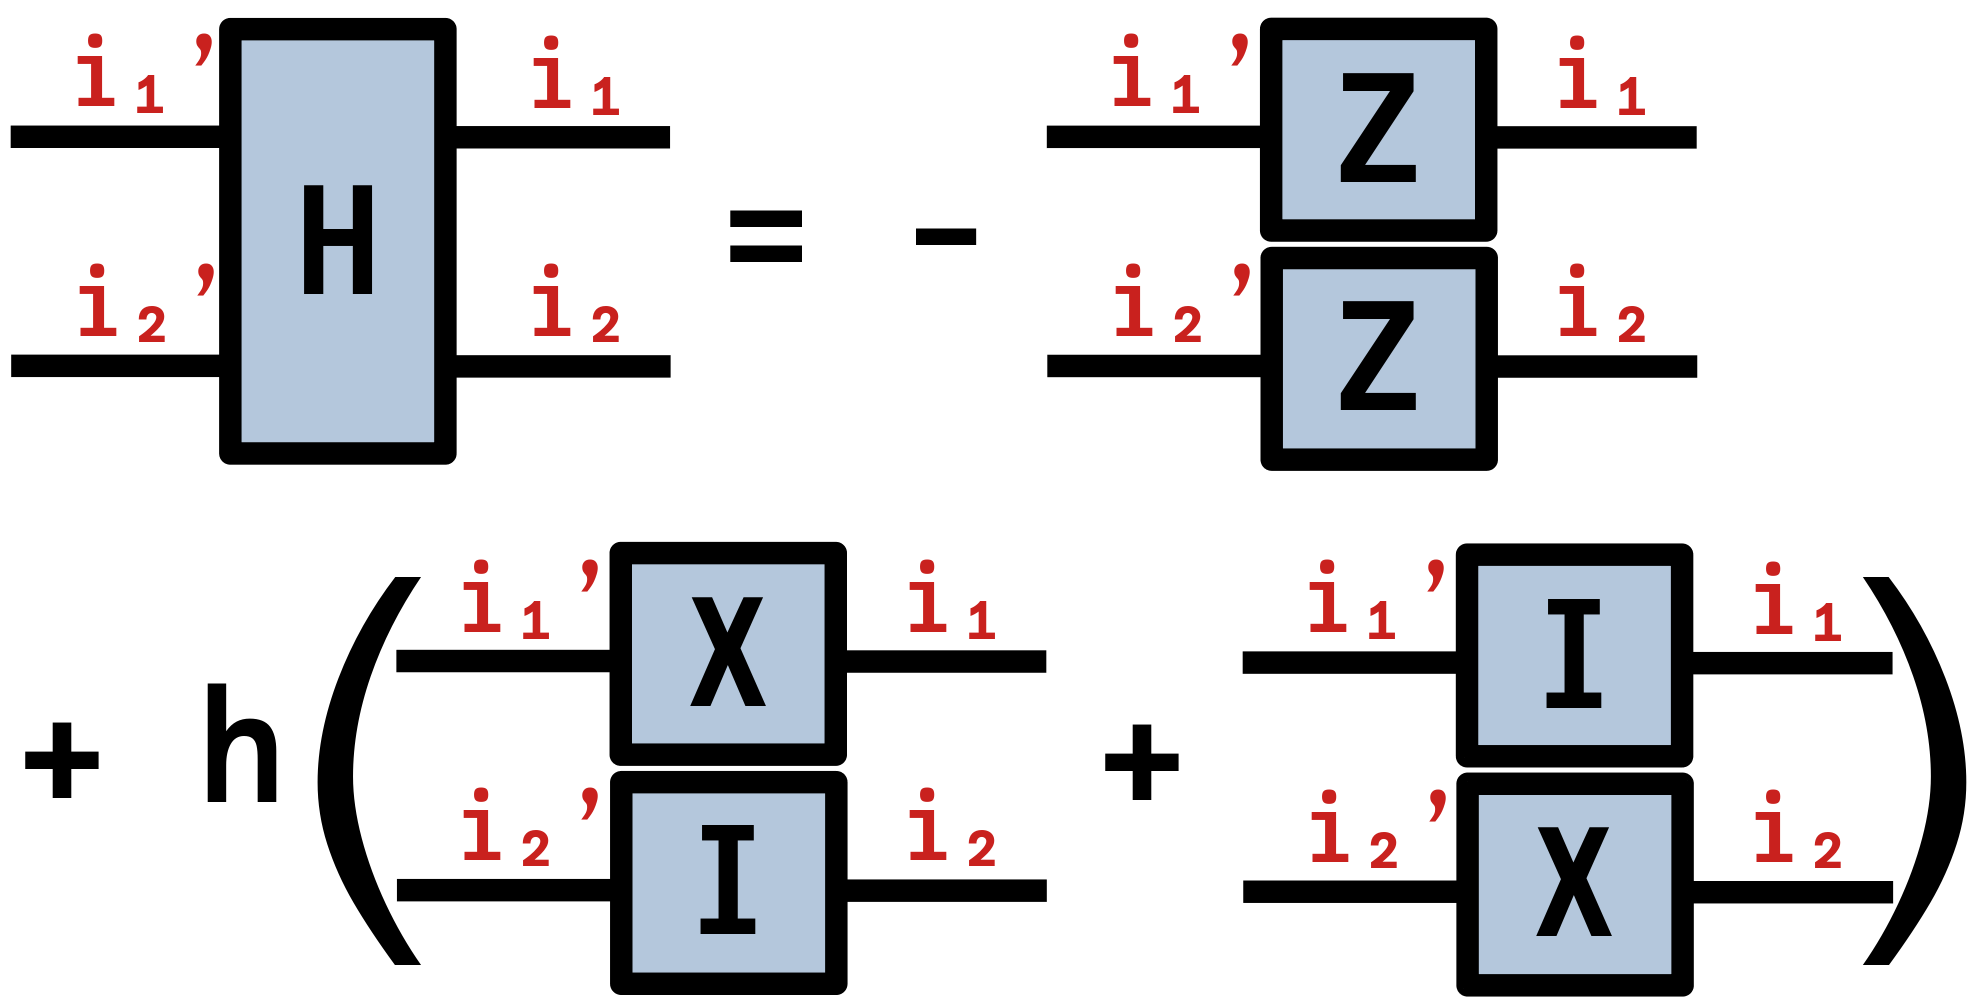
\includegraphics[width=1.0\textwidth]{
  slides/assets/ising12.png
}
\end{center}
\vspace*{0.0cm}
\end{onlyenv}

\end{column}

\end{columns}

\end{frame}
